\documentclass{beamer}
\usepackage[utf8]{inputenc}

\usetheme{Madrid}
\usecolortheme{default}
\usepackage{extarrows}
\usepackage{amsmath}
\usepackage{extarrows}
\usepackage{amssymb,amsfonts,amsthm}
\usepackage{txfonts}
\usepackage{tkz-euclide}
\usepackage{listings}
\usepackage{adjustbox}
\usepackage{array}
\usepackage{tabularx}
\usepackage{gvv}
\usepackage{lmodern}
\usepackage{circuitikz}
\usepackage{tikz}
\usepackage{graphicx}
\usepackage{amsmath} 

\setbeamertemplate{page number in head/foot}[totalframenumber]

\usepackage{tcolorbox}
\tcbuselibrary{minted,breakable,xparse,skins}

\definecolor{bg}{gray}{0.95}
\DeclareTCBListing{mintedbox}{O{}m!O{}}{%
  breakable=true,
  listing engine=minted,
  listing only,
  minted language=#2,
  minted style=default,
  minted options={%
    linenos,
    gobble=0,
    breaklines=true,
    breakafter=,,
    fontsize=\small,
    numbersep=8pt,
    #1},
  boxsep=0pt,
  left skip=0pt,
  right skip=0pt,
  left=25pt,
  right=0pt,
  top=3pt,
  bottom=3pt,
  arc=5pt,
  leftrule=0pt,
  rightrule=0pt,
  bottomrule=2pt,
  toprule=2pt,
  colback=bg,
  colframe=orange!70,
  enhanced,
  overlay={%
    \begin{tcbclipinterior}
    \fill[orange!20!white] (frame.south west) rectangle ([xshift=20pt]frame.north west);
    \end{tcbclipinterior}},
  #3,
}
\lstset{
    language=C,
    basicstyle=\ttfamily\small,
    keywordstyle=\color{blue},
    stringstyle=\color{orange},
    commentstyle=\color{green!60!black},
    numbers=left,
    numberstyle=\tiny\color{gray},
    breaklines=true,
    showstringspaces=false,
}
\title %optional
{10.4.8}


\author 
{Kartik Lahoti - EE25BTECH11032}

\begin{document}


\frame{\titlepage}
\begin{frame}{Question}
For which value of $m$ is the line
\begin{align}
    y = mx + 1
\end{align}
a tangent to the curve 
\begin{align}
    y^2 = 4x
\end{align}

\end{frame}

\begin{frame}{Theoretical Solution}
Given parabola 
\begin{align}
    g\brak{\vec{x}} = \vec{x}^{\top}\vec{V}\vec{x} + 2\vec{u}^{\top}\vec{x} + f = 0 \\
    \vec{V} = \myvec{0&0\\0&1} , \vec{u} = \myvec{-2\\0} , f = 0.
\end{align}
Given Line equation
\begin{align}
    \vec{x} = \vec{h} + k\vec{m}\\
    \vec{h} = \myvec{0\\1} , \vec{m} = \myvec{1 \\ m}.
\end{align}
\end{frame}

\begin{frame}{Theoretical Solution}
For the line to be a tangent , all the solution for $k$ should be equal

\begin{align}
    k_i = \frac{1}{\vec{m}^{\top}\vec{V}\vec{m}}\brak{-\vec{m}^{\top}\brak{\vec{V}\vec{h}+\vec{u}} \pm \sqrt{\sbrak{\vec{m}^{\top}\brak{\vec{V}\vec{h}+\vec{u}}}^2-g\brak{\vec{h}}\brak{\vec{m}^{\top}\vec{V}\vec{m}}}} \label{eq_1}
\end{align}

From \ref{eq_1} 
\begin{align}
    \sbrak{\vec{m}^{\top}\brak{\vec{V}\vec{h}+\vec{u}}}^2 = g\brak{\vec{h}}\brak{\vec{m}^{\top}\vec{V}\vec{m}} \label{eq_3}
\end{align}
\end{frame}

\begin{frame}{Theoretical Solution}
\begin{align}
    g\brak{\vec{h}} = \myvec{0&1}\myvec{0&0\\0&1}\myvec{0\\1} + 2\myvec{-2&0}\myvec{0\\1} + 0 = 1 \label{eq_2}
\end{align}

Using \ref{eq_2} in \ref{eq_3}

\begin{align}
    \sbrak{\myvec{1 & m }\brak{\myvec{0&0\\0&1}\myvec{0\\1} + \myvec{-2\\0}}}^2 = 1\brak{\myvec{1&m}\myvec{0&0\\0&1}\myvec{1\\m}}
\end{align}
\end{frame}
\begin{frame}{Theoretical Solution}
\begin{align}
    \implies \brak{m-2}^2 &= m^2 \\ 
    \implies 4 - 4m &=   0 \\ 
    \implies m &= 1
\end{align}
\end{frame}

 \begin{frame}{Plot}
    \centering
    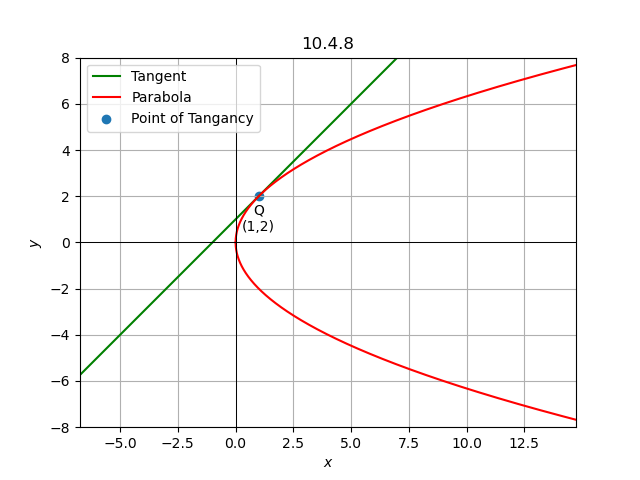
\includegraphics[width=\columnwidth, height=0.8\textheight, keepaspectratio]{../figs/graph1.png}   
\end{frame}

\end{document}
